\chapter{Introdução a Luderia}
\label{chap:intro}

Uma luderia é uma loja que aluga e vende jogos. Normalmente, esse tipo de negócio inclui um bar ou restaurante, que atende os fregueses, monitores que ensinam a jogar e possivelmente outras atividades. 

O aluguel de jogos é basicamente um diferencial de atração, não sendo a única fonte de renda, que é o consumo no bar e restaurante. Porém, ele também tem que dar lucro, além de exigir um trabalho de curadoria e monitoria, como veremos neste documento.

Esse documento descreve o funcionamento da Luderia SemNome, que é feito todo de forma manual, usando papel e caneta. A suposição é que todo serviço será informatizado, em vários módulos que comporão um sistema único.

Basicamente, uma luderia pode funcionar com diferentes modelos de negócio: cobrar ingresso, cobrar consumo mínimo, cobrar pelo aluguel dos jogos, ou um mix desses modelos. A Luderia SemNome trabalha com o modelo de ingresso, mas quer ter liberdade para mudar esse modelo em qualquer momento, ou variar o modelo por dia.

Este documento serve de referência para exercícios de Engenharia de Software, da especificação de serviço ao desenvolvimento, teste e manutenção, de um sistema de informação que apoia todas as suas funções de negócio.

\section{Serviços prestados na Luderia}

A Luderia SemNome oferece os seguintes serviços, que serão tratados de forma detalhada mais adiante no texto:
\begin{enumerate}
    \item uma recepção (Capítulo \ref{chap:recepcao});
    \item empréstimo (Capítulo \ref{chap:aluguel}), no local, de jogos de tabuleiro e cartas;
    \item atendimento com bebidas (Capítulo \ref{chap:barest}), incluindo refrigerantes, bebidas alcoólicas, drinks com ou sem álcool e sucos naturais, feitas no bar;
    \item atendimento com comidas (Capítulo \ref{chap:barest}), incluindo lanches, como sanduíches e pizza, aperitivos, como porções de batata-frita, pratos feitos, como filé com fritas, feitas na cozinha;
    \item garçons ou \textit{self-service} (Capítulo \ref{chap:barest}), conforme a escolha do cliente;
    \item uma grande área com mesas onde se pode jogar ou consumir alimentos e bebidas;
    \item monitoria (Capítulo \ref{chap:monitor}), com monitores que ensinam a jogar os jogos, e a ainda outras formas de apoio ao jogador, como mestres cadastrados e professores;
    \item um clube de membros (Capítulo \ref{chap:clube});
    \item uma loja (Capítulo \ref{chap:loja}), onde se podem comprar jogos de tabuleiro e cartas, além de acessórios;
    \item aluguel de jogos, que permite que o cliente leve o jogo para casa;
    \item um setor de entregas, que entrega comidas e jogos, emprestados ou vendidos;
    \item um caixa único, na saída da Luderia;
    \item a gerência de RH, responsável pelo pessoal;
    \item a gestão financeira, que controla o resultado;
    \item o estoque da loja (Capítulo \ref{chap:loja});
    \item o estoque de empréstimos, que fica localizado em uma parede da loja, e
    \item o estoque de bebidas e alimentos, prontos ou insumos.
    \rafael{ Não sei se valeria incluir a pessoa responsável por lidar com as editoras para comprar jogos novos.}
\end{enumerate}


\section{Horário de Funcionamento e Cobrança}

Os horários de funcionamento da Luderia e como é cobrado o ingresso, estão descritos na Tabela \ref{tab:ludehorarios}. Detalhes da forma de aluguel atual e planos para o futuro são descritos no Capítulos \ref{chap:aluguel}. Os horários podem mudar no futuro.

\begin{table}[hbt]
    \centering
    \begin{tabular}{cccc}
    \toprule
    dia & início & fim & cobrança\\
    \midrule
        segunda & \multicolumn{3}{c}{não funciona} \\
         terça & 13:00 & 22:00 & ingresso grátis \\
         quarta e quinta & 13:00 & 22:00 & ingresso com desconto cobrado 50\%\\
         sexta e sábado & 12:00 & 24:00 & ingresso normal \\
         domingo & 12:00 & 21:00 & ingresso normal \\
    \bottomrule
    \end{tabular}
    \caption{Horários da Luderia}
    \label{tab:ludehorarios}
\end{table}

\section{Como é a Luderia}

A Luderia tem como espaço físico uma grande casa de três andares, que permite dividir de forma adequada os serviços, de acordo com o seguinte quadro:
\begin{itemize}
    \item hall, onde estão 3 balcões: recepção, balcão de empréstimos e caixa;
    \item loja, em um salão no térreo acessado pelo hall;
    \item salas de mesa, uma sala no primeiro e duas segundo andar;
    \item um salão para reservas, dedicado a festas ou eventos privados, no terceiro andar;
    \item ludoteca, uma pequena sala no primeiro andar com estantes com jogos e uma mesa para permitir que os clientes os abram, além de um balcão de aluguel. \rafael{ No caso da Ludus, que é a maior que conheço, isso fica numa vitrine, mas o cliente não toca nisso. Ele pode até apontar e pedir para um monitor pegar, mas quem manuseia e lida com os jogos antes de irem pra mesa é o monitor.}
    \item bar, um balcão grande no primeiro andar, que permite fazer drinks e sucos, e um balcão de apoio no segundo andar;
    \item cozinha, no primeiro andar;
    \item banheiros, masculino e feminino, no primeiro e segundo andares;
    \rafaelx{ A Game of Boards aboliu os gêneros. Agora os banheiros são mistos.}
    \item gerência, vestiário, banheiros dos funcionários, no terceiro andar, e 
    \item um depósito, em uma outra construção fora da casa.
    \end{itemize}

Uma escada liga todos os andares. Não há elevador, porém a escada possui um dispositivo que permite que uma pessoa com dificuldades se sente e seja levado.

Só é possível sair da Luderia passando pela loja. Existe um elevador de alimentos da cozinha para o segundo andar, mas não para o terceiro.

\begin{figure}[hbt]
    \centering
    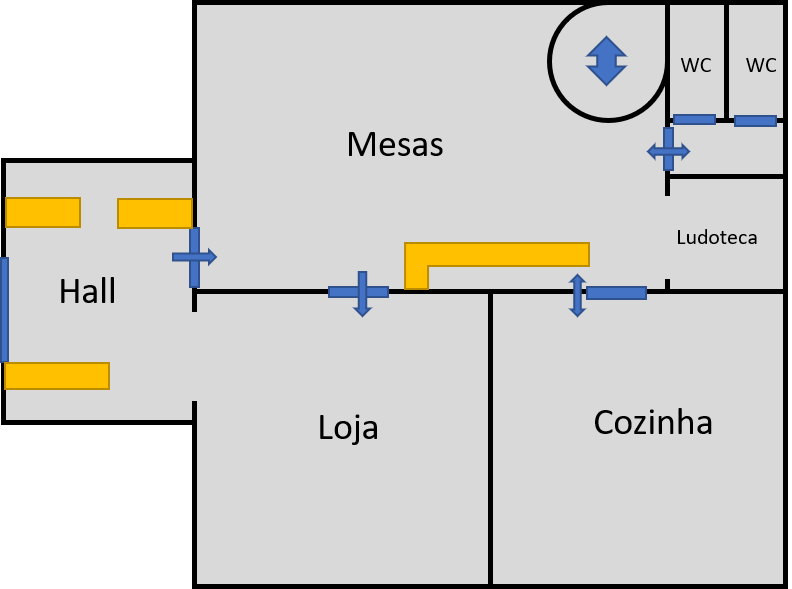
\includegraphics[scale=0.8]{imagens/PrimeiroAndar.png}
    \caption{Primeiro andar da Luderia}
    \label{fig:andar1}
\end{figure}

\begin{figure}[hbt]
    \centering
    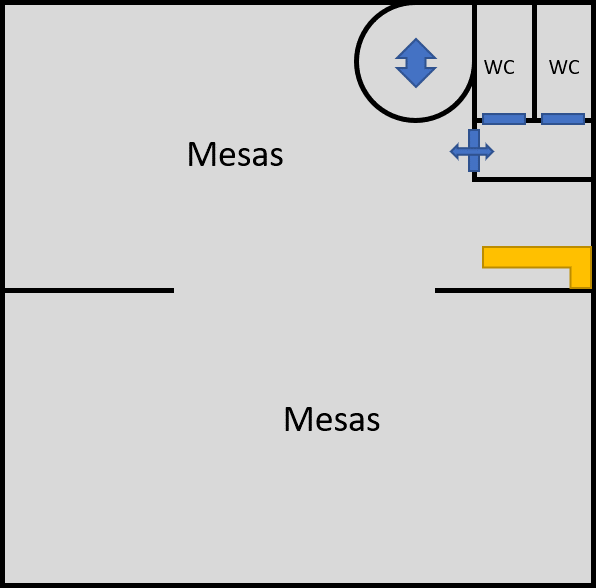
\includegraphics[scale=0.8]{imagens/SegundoAndar.png}
    \caption{Segundo andar da Luderia}
    \label{fig:andar2}
\end{figure}

\begin{figure}[hbt]
    \centering
    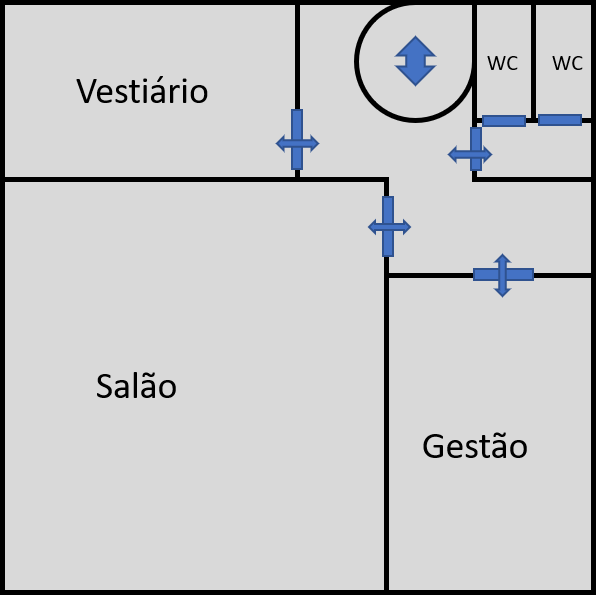
\includegraphics[scale=0.8]{imagens/TerceiroAndar.png}
    \caption{Terceiro andar da Luderia}
    \label{fig:andar3}
\end{figure}

\section{O atendimento atual}

O atendimento atual é todo feito na mão, com um cartão de consumo de papel onde os funcionários anotam as compras.

Esse cartão traz vários problemas. Se perdido, não se sabe quanto a pessoa consumiu. Os funcionários têm letra ruim, dificultando a vida do caixa.

Eles ainda amassam, molham e devem ser impressos frequentemente, ou guardados, se impressos em grande quantidade.


\section{O cartão de consumo de plástico}

A empresa decidiu que o sistema deverá usar um cartão de consumo de plástico, e já os comprou.

O cartão de consumo a ser usado contém um número e um QR-Code que representa esse número. Todos os funcionários da Luderia carregarão um equipamento (mini-tablet) que permitirá usar o sistema a ser construído para registrar pedidos na conta do cliente, bastando para isso scannear o cartão ou usar o número que está nele impresso.
\rafaelx{ Diria que esse número é em alto relevo, caso contrário, com o manuseio, o QR code e os dígitos ficarão desgastados.}

A Luderia comprou um pacote de 1000 cartões, mesmo que não caibam tantas pessoas na casa.

\section{A questão do barulho, brigas e assédio}

A Luderia é destinada a jogos de sociedade que fazem barulho naturalmente. Jogos que exigem silêncio podem ser jogados, quando disponível, isto é, não estiver sendo alugado, no salão do terceiro andar. Nesse caso, o comportamento no local deve ser de máximo esforço para o silêncio, sendo apenas permitidas conversas exigidas pelo jogo.

Barulho excessivo, porém, poderá ser controlado pelos monitores. Brigas serão imediatamente interrompidas pelo monitor responsável pela sala. A violência física significa o banimento do jogador da Luderia. Deve haver registro do jogador banido em qualquer sistema futuro.

O assédio moral e sexual também é causa de banimento.

\section{Proibições e Permissões}

Não é permitido o jogo com apostas. 

Em geral, também não é permitido trazer bebidas e comidas de fora, sendo que exceções são feitas para alimentação de crianças pequenas.

Grupos trazem seu próprio jogo estão sujeitos a pagar a consumação mínima, ou pagar a taxa de aluguel de jogos mais baratos, dependendo da forma de cobrança. Se a cobrança for por ingresso, isto não será necessário.

\section{Pedidos gerais sobre a implementação}

O sistema informatizado deve ter as seguintes características, segundo os proprietários:
\begin{itemize}
    \item ser um sistema único e integrado;
    \item usar uma base de dados open-source, gratuita e única;
    \item ter uma interface de usuário com programação única, via web, e que se adapte aos vários dispositivos que vão ser usados, podendo ser acessado via: celulares, tablets e computadores, como telas de diferentes tamanhos;
    \item parte do sistema deverá ser acessada diretamente pelos clientes;
    \item ter uma interface com serviços de emissão de nota fiscal, e
    \item usar linguagens de programação gratuitas e abertas.
\end{itemize}

\rafael{ O que você acha dos membros cadastrados na plataforma, mesmo que não paguem mensalidade, poderem consultar antecipadamente se um determinado jogo está na loja, antes da pessoa ter que se deslocar até lá.}

